% =============================================================================
% CalRank: Calibration of Cross-Encoder Re-Rankers
% Format-neutral manuscript: standard article class, common packages only.
% Compiles as-is (pdflatex calrank.tex).
%
% ADAPTING TO A TARGET JOURNAL AT SUBMISSION:
%   * JISE  : two-column; paste body into the JISE template, keep \section order.
%   * ComSIS: download the ComSIS LaTeX class, replace the preamble below with
%             \documentclass{comsis}, keep everything from \begin{document} on.
% The content, tables, and figure calls are template-independent.
% =============================================================================
\documentclass[11pt,a4paper]{article}

\usepackage[utf8]{inputenc}
\usepackage[T1]{fontenc}
\usepackage{lmodern}
\usepackage[margin=1in]{geometry}
\usepackage{amsmath,amssymb}
\usepackage{graphicx}
\usepackage{booktabs}
\usepackage{multirow}
\usepackage{array}
\usepackage{siunitx}
\usepackage[table]{xcolor}
\usepackage[hidelinks]{hyperref}
\usepackage{caption}
\usepackage{microtype}
\usepackage{enumitem}

\graphicspath{{../data/figures/}}

\sisetup{detect-weight=true,detect-family=true}
\newcommand{\ece}{\mathrm{ECE}}
\newcommand{\sigmoid}{\sigma}

% Table colours
\definecolor{headblue}{HTML}{2C3E6B}
\definecolor{rowlight}{HTML}{EAF0FA}
\definecolor{rowwhite}{HTML}{FFFFFF}
\definecolor{cleangreen}{HTML}{E6F5E8}
\definecolor{singleclasspink}{HTML}{FDE8E8}
\definecolor{bestcell}{HTML}{D5F5E3}
\newcommand{\thead}[1]{\textcolor{white}{\textbf{#1}}}

\title{\bfseries How Calibrated Are Cross-Encoder Re-Rankers?\\
An Empirical Study and a Cautionary Tale}

\author{%
  Sayanjib [Surname]\\
  \small [Affiliation]\\
  \small \texttt{[email]}
}
\date{}

\begin{document}
\maketitle

% =============================================================================
\begin{abstract}
\noindent
Cross-encoder re-rankers are quietly being asked to do something they were never
trained for. Originally designed to sort documents by relevance, their sigmoid scores
now serve as probability estimates in retrieval-augmented generation pipelines,
abstention layers, and multi-stage cascades. Nobody, to our knowledge, has checked
whether those probabilities mean what they claim to mean. We set out to answer that
question. Across five small cross-encoder models (4M to 278M parameters) and nine
BEIR-family domains, we measure Expected Calibration Error, Maximum Calibration
Error, and Brier score with bootstrap confidence intervals. The short answer is that
every model is overconfident, often dramatically so; optimal temperatures range from
about three to above twenty. But the longer answer is more troubling. Most BEIR
datasets carry only positive relevance judgments, and this quietly corrupts
calibration evaluation, making temperature scaling look unreliable when it is not. On
the four datasets that do contain genuine negatives, temperature scaling, Platt
scaling, and isotonic regression all reduce calibration error significantly, with
isotonic regression dominating, and none of them disturb the ranking. We release the
scored pairs, fitted calibrators, and code.
\medskip

\noindent\textbf{Keywords:} calibration; cross-encoder re-ranking; information
retrieval; expected calibration error; temperature scaling; isotonic regression;
BEIR; retrieval-augmented generation.
\end{abstract}

% =============================================================================
\section{Introduction}
\label{sec:intro}

A cross-encoder re-ranker reads a query alongside a candidate document and produces
a score. Sort by score, and you have a ranking. That is what these models were built
for, and they do it well. What is newer, and less examined, is the growing practice
of reading that score as a probability. Consider a retrieval-augmented assistant that
only forwards passages scoring above $p=0.7$ to its language model generator. Or an
abstention system that refuses to answer when nothing in the retrieved pool looks
confident enough. Or a cascade where low-scoring queries get routed to a bigger,
costlier model~\cite{lewis2020rag,gao2024rag}. In each of these cases, the
$\sigmoid(\text{logit})$ output is being consumed as if it were
$P(\text{relevant}\mid q,d)$. A score of 0.7 is treated as meaning: there is a
seventy percent chance this document is relevant.

Whether that trust is warranted is, frankly, an open question. These models learn
from MS~MARCO~\cite{nguyen2016msmarco} with objectives that reward getting the
ordering right. Separation is what matters during training: relevant above
non-relevant. Probabilistic accuracy is a different property
entirely~\cite{degroot1983}, and a model can excel at one while failing at the other.
There is no free theorem that connects ranking quality to calibration. So when a
production pipeline reads 0.7 as seventy percent, it is making an assumption that
nobody has systematically tested.

The calibration literature has covered image classifiers in some
depth~\cite{guo2017}, and there is growing attention to large language
models~\cite{kadavath2022,jiang2021}. Cross-encoder re-rankers, despite being
deployed at scale as de facto probability estimators, have mostly escaped scrutiny.
No systematic study has looked at how their scores behave as probabilities across
domains, no per-domain picture exists, and there is no empirical guidance on which
post-hoc fix a practitioner should reach for. We set out to fill that gap, and in the
process we stumbled onto a second, arguably more interesting problem: a structural
issue with how calibration is evaluated on standard IR benchmarks.

What follows is, in essence, two interleaved contributions. The empirical one charts
the calibration landscape. The methodological one explains why a naive reading of
that landscape leads to wrong conclusions. Specifically:

\begin{itemize}[leftmargin=*,itemsep=2pt]
  \item \textbf{C1.} We conduct, to our knowledge, the first systematic calibration
  study of small cross-encoder re-rankers: five models spanning 4M to 278M
  parameters across nine BEIR-family domains, with ECE, MCE, and Brier score
  supported by bootstrap confidence intervals (Section~\ref{sec:overconf},
  Figure~\ref{fig:grid}, Table~\ref{tab:raw}).

  \item \textbf{C2.} We uncover a methodological hazard. Five of the nine datasets
  carry only positive relevance judgments, a prevalence of exactly 1.0, and this
  silently makes calibration evaluation degenerate. Temperature scaling appears
  unreliable on these datasets, but the problem is the evaluation, not the method
  (Section~\ref{sec:hazard}, Table~\ref{tab:datasets}).

  \item \textbf{C3.} Restricting to datasets with genuine negatives, we find that all
  three post-hoc methods work, with a clear ordering: isotonic beats Platt, which
  beats temperature. Ranking quality is preserved to within $10^{-4}$ in nDCG@10
  (Sections~\ref{sec:clean}--\ref{sec:downstream}, Tables~\ref{tab:clean}--\ref{tab:downstream}, Figure~\ref{fig:cleangrid}).

  \item \textbf{C4.} We release scored pairs, fitted per-model calibrators as a
  deployment recipe (Table~\ref{tab:recipe}), reliability diagrams, and code.
\end{itemize}

One thing worth stating upfront: we are not claiming that temperature scaling fails.
Our own analysis, done carefully, shows it works. The claim is subtler than that.
What looks like failure is actually an artifact of dataset structure, and the
structure has to be reported for any calibration number on these benchmarks to carry
meaning.

The rest of the paper follows a conventional arc. Section~\ref{sec:related} reviews
the relevant background. Section~\ref{sec:method} describes the experimental setup,
with particular attention to the choices we made and why. Section~\ref{sec:results}
presents the findings, which are organised around four observations.
Section~\ref{sec:sensitivity} tests how sensitive our conclusions are to the
treatment of unjudged documents. Sections~\ref{sec:discussion} and~\ref{sec:limits}
discuss implications and limitations, and Section~\ref{sec:conclusion} wraps up.

% =============================================================================
\section{Background and Related Work}
\label{sec:related}

\subsection{Cross-encoder re-rankers}
The two-stage retrieval pipeline has become something of a standard
recipe~\cite{nogueira2019}. A fast first-stage system, typically BM25 or a learned
sparse retriever~\cite{robertson2009bm25}, produces a rough candidate pool. Then a
cross-encoder re-ranks that pool by reading each query-document pair jointly through
a transformer. The joint encoding is what gives cross-encoders their edge over
bi-encoders~\cite{reimers2019sbert}, which embed query and document in separate
passes and can only interact through a similarity function. Cross-encoders see both
sides at once, which lets them model token-level interactions that bi-encoders miss.

Nogueira and Cho~\cite{nogueira2019} were among the first to fine-tune BERT for
passage re-ranking on MS~MARCO, and the approach quickly branched into a family of
variants. MiniLM~\cite{wang2020minilm} and TinyBERT~\cite{jiao2020tinybert} distil
the knowledge of larger teachers into compact students, trading a bit of accuracy for
substantially faster inference. ELECTRA~\cite{clark2020electra} brings a different
pretraining recipe, replaced-token detection, that can extract more from the same
parameter budget. The BGE family~\cite{xiao2023bge} builds on XLM-RoBERTa with
additional contrastive learning. What all these models share is a single logit output,
conventionally mapped through a sigmoid to produce a number between zero and one.
That number is what downstream systems interpret as a probability.

\subsection{What calibration means, and how to measure it}
A predictor is calibrated when it means what it says~\cite{degroot1983}. If it
outputs 0.8 for a thousand predictions, roughly eight hundred of those should turn
out to be correct. Expected Calibration Error, or ECE~\cite{naeini2015}, tries to
measure the gap between confidence and reality by binning predictions into groups and
averaging the per-bin difference, weighted by how many predictions land in each bin.
It is the most commonly reported metric, though it comes with caveats: the number of
bins matters, and different binning schemes can give different
answers~\cite{nixon2019,kumar2019}. We use fifteen equal-width bins throughout, and
we treat that as a fixed methodological choice rather than tuning it.

Maximum Calibration Error (MCE) picks out the single worst bin, a useful complement
when you care about the tails. The Brier score~\cite{brier1950} takes a different
approach entirely: it is the mean squared error between the predicted probability and
the binary outcome, which makes it a proper scoring rule that rewards both
calibration and discrimination simultaneously. Reliability
diagrams~\cite{degroot1983,niculescu2005} put the same information into visual form,
plotting empirical accuracy against predicted confidence for each bin. A well-calibrated
model traces the diagonal; bars that fall below it signal overconfidence.

\subsection{Fixing calibration after the fact}
Temperature scaling~\cite{guo2017} is the simplest post-hoc fix. You learn a single
scalar $T$ and divide the logit by it before applying the sigmoid. When $T>1$, which
is the usual case for overconfident models, the probabilities get softened. The whole
thing is a monotone transform, so the ranking stays exactly the same. Guo et al.\
showed that this one-parameter trick is surprisingly effective for deep image
classifiers, and it has since become the default first-line correction in much of the
literature.

Platt scaling~\cite{platt1999} adds a second parameter. Instead of just scaling the
logit, it fits a logistic regression on it, learning both a slope and an intercept.
The intercept lets it shift the decision boundary, which temperature alone cannot do.
It is still monotone. Isotonic regression~\cite{zadrozny2002} goes further, fitting
a non-parametric step function via the pool-adjacent-violators algorithm. It can
match any monotone shape, which makes it powerful but also makes it more susceptible
to overfitting on small datasets. What matters for our purposes is that all three
transforms are monotone: they cannot reorder documents, so calibration, in principle,
is free from a ranking perspective.

\subsection{Calibration beyond classifiers}
The calibration literature started with weather forecasting~\cite{brier1950} and
found renewed energy when Guo et al.~\cite{guo2017} showed that modern deep
networks are often more overconfident than their shallower predecessors. More
recently, large language models have drawn attention. Kadavath et
al.~\cite{kadavath2022} investigated whether LLMs ``know what they know,'' and Tian
et al.~\cite{tian2023} explored strategies for eliciting better-calibrated
confidence from RLHF-tuned models. In NLI, Desai and Durrett~\cite{desai2020} found
that fine-tuned BERT is reasonably well-calibrated in-domain but degrades under
distribution shift.

In information retrieval specifically, the picture is sparse. Craswell et
al.~\cite{craswell2020} and Lin et al.~\cite{lin2021pyserini} evaluated neural
re-rankers on BEIR and MS~MARCO, but their focus was ranking effectiveness, not
whether the probability estimates themselves are trustworthy. The selective prediction
literature~\cite{geifman2017,el2010} is conceptually adjacent: systems that abstain
when uncertain depend on well-calibrated confidence, though this connection is rarely
made explicit in IR work. To our knowledge, nobody has conducted a systematic
cross-domain calibration study of cross-encoder re-rankers. That is where we come in.

% =============================================================================
\section{Methodology}
\label{sec:method}

\subsection{Models}
\label{sec:models}
We study five publicly available cross-encoder re-rankers, listed in
Table~\ref{tab:models}. The selection was deliberate on two axes. On scale, they
range from 4M parameters (TinyBERT-L2) to 278M (BGE-reranker), which spans the
range one actually encounters in latency-sensitive deployments. On architecture, they
cover distilled BERT variants, ELECTRA's replaced-token-detection approach, and
XLM-RoBERTa. The idea was to see whether calibration behaviour tracks with model
family, model size, or neither.

We intentionally confined ourselves to small models. Larger re-rankers certainly
exist, and they are interesting in their own right, but the small ones are what
engineers actually deploy when milliseconds matter. That makes them the natural
objects of a calibration study aimed at practitioners. One model we had hoped to
include, jina-reranker-v1-tiny-en, turned out to be incompatible with
\texttt{transformers}~$\geq 5.0$ due to removed internal APIs, so we excluded it.

\begin{table}[t]
\centering
\caption{The five cross-encoder re-rankers studied.}
\label{tab:models}
\small
\begin{tabular}{llrl}
\toprule
\rowcolor{headblue}
\thead{Key} & \thead{HuggingFace model} & \thead{Params} & \thead{Architecture} \\
\midrule
\rowcolor{rowlight}
TinyBERT-L2  & cross-encoder/ms-marco-TinyBERT-L-2-v2 & 4M   & 2-layer TinyBERT \\
\rowcolor{rowwhite}
MiniLM-L6    & cross-encoder/ms-marco-MiniLM-L-6-v2   & 22M  & 6-layer MiniLM \\
\rowcolor{rowlight}
MiniLM-L12   & cross-encoder/ms-marco-MiniLM-L-12-v2  & 33M  & 12-layer MiniLM \\
\rowcolor{rowwhite}
ELECTRA-base & cross-encoder/ms-marco-electra-base    & 110M & ELECTRA-base \\
\rowcolor{rowlight}
BGE-reranker & BAAI/bge-reranker-base                 & 278M & XLM-RoBERTa-base \\
\bottomrule
\end{tabular}
\end{table}

\subsection{Datasets}
\label{sec:datasets}
We use nine datasets drawn from the BEIR family~\cite{thakur2021beir}. They are
summarised in Table~\ref{tab:datasets}, and the table is ordered by prevalence,
the fraction of judged pairs that carry a positive label, because that ordering
turns out to be the most important thing in this paper.

Look at the prevalence column. The first four datasets have some real negatives:
dbpedia-entity sits at 0.35, trec-covid at 0.62, webis-touche2020 at 0.78, and
scidocs at 0.95. Then there is a wall: the remaining five datasets all show a
prevalence of exactly 1.00. Every single judged pair is relevant. The reason is
simple but consequential: these collections were annotated by marking known relevant
documents against queries, and documents not marked were left unjudged rather than
being labelled non-relevant. The result is that judged-only evaluation on these
datasets has no negative examples to work with, and as we will see in
Section~\ref{sec:hazard}, this silently breaks calibration assessment.

We added dbpedia-entity to the original eight precisely because we needed a
well-balanced anchor. It is the only large-scale BEIR set with graded judgments and
a substantial pool of genuine negatives: 9{,}182 judged pairs across 400 queries,
with about two thirds of them non-relevant. Without it, the study would rest on just
three datasets with real negatives, two of which (webis-touche2020 and scidocs)
have their own issues. More on that in Section~\ref{sec:limits}.

\begin{table}[t]
\centering
\caption{Datasets, ordered by positive prevalence. Judged pairs are counted among
the BM25 top-100. Five datasets carry only positive judgments
(prevalence $=1.00$), which corrupts calibration evaluation
(Section~\ref{sec:hazard}).
\textcolor{green!50!black}{Green}: clean subset (real negatives).
\textcolor{red!50!black}{Pink}: positive-only judgments.}
\label{tab:datasets}
\small
\begin{tabular}{llrrrr}
\toprule
\rowcolor{headblue}
\thead{Dataset} & \thead{Domain} & \thead{\#Queries} & \thead{Corpus} & \thead{\#Judged} & \thead{Prevalence} \\
\midrule
\rowcolor{cleangreen}
dbpedia-entity   & Entity retrieval     & 400   & 4{,}635{,}922 & 9{,}182 & 0.35 \\
\rowcolor{cleangreen}
trec-covid       & Biomedical           & 50    & 171{,}332     & 3{,}475 & 0.62 \\
\rowcolor{cleangreen}
webis-touche2020 & Argument retrieval   & 49    & 382{,}545     & 635     & 0.78 \\
\rowcolor{cleangreen}
scidocs          & Scientific citation  & 1{,}000 & 25{,}657    & 1{,}774 & 0.95 \\
\rowcolor{singleclasspink}
arguana          & Counter-arguments    & 1{,}406 & 8{,}674     & 1{,}316 & 1.00 \\
\rowcolor{singleclasspink}
fiqa             & Financial QA         & 648   & 57{,}638      & 756     & 1.00 \\
\rowcolor{singleclasspink}
nfcorpus         & Health               & 323   & 3{,}633       & 1{,}941 & 1.00 \\
\rowcolor{singleclasspink}
quora            & Duplicate questions  & 1{,}000 & 522{,}931   & 1{,}278 & 1.00 \\
\rowcolor{singleclasspink}
scifact          & Scientific claims    & 300   & 5{,}183       & 298     & 1.00 \\
\bottomrule
\end{tabular}
\end{table}

\subsection{Pipeline}
\label{sec:pipeline}
The pipeline follows the standard two-stage recipe. For each query we retrieve the
top 100 documents using BM25, implemented via \texttt{bm25s}~\cite{bm25s2024} with
$k_1=0.9$ and $b=0.4$. We went with a pure-Python implementation to avoid the JVM
dependency that comes with Anserini, which makes the whole thing reproducible on a
laptop. Top-100 is the standard cutoff for re-ranking and mirrors what you would see
in deployment.

Each candidate pair is then scored by all five cross-encoders. For every scored pair
we store three things: the raw logit, its sigmoid, and a binarised relevance label
from the qrels ($-1$ for unjudged, $0$ for judged non-relevant, $1$ for judged
relevant). Quora was subsampled to 1{,}000 queries for cost. All scoring ran on an
Apple~M4 with the Metal Performance Shaders backend. The full pipeline produces
roughly twenty thousand judged pairs per model across the nine datasets, drawn from
about half a million scored pairs including the unjudged ones. Results are written
atomically per model-dataset pair, so the pipeline is resumable if it gets
interrupted.

\subsection{Metrics and uncertainty}
\label{sec:metrics}
We compute ECE, MCE, and Brier score on judged pairs only, using fifteen equal-width
bins. To quantify uncertainty, we attach a 95\% confidence interval to ECE via a
query-level bootstrap with 1{,}000 resamples. This is not something every
calibration study does, and we think it should be, especially on datasets with few
queries.

We deliberately left AUC out. On the single-class datasets it is undefined, and even
where it is defined, discrimination is simply not the question we are asking. A model
can rank perfectly and still assign probabilities that are wildly
off~\cite{degroot1983}. Including AUC would muddy the story without adding clarity.

\subsection{Post-hoc calibration protocol}
\label{sec:protocol}
For each model-dataset pair, we split the judged pairs 50/50, stratified by label,
with a fixed seed of 42. Temperature, Platt, and isotonic calibrators are fit on one
half and evaluated on the other. The held-out evaluation is particularly important
for isotonic regression, which can memorise the distribution of its fit data and
report ECE values that look implausibly good. Every calibrated ECE in this paper
comes from the held-out test split, and this matters enough that we will say it once
more: no calibrator was ever evaluated on the data it was trained on.

Where stratification fails because there is only one class, we fall back to random
splitting. This happens on the five prevalence-one datasets and, as we shall see,
those splits are not very informative anyway.

% =============================================================================
\section{Results}
\label{sec:results}

\subsection{Re-rankers are severely and universally overconfident}
\label{sec:overconf}

Figure~\ref{fig:grid} tells the story at a glance. It shows raw reliability diagrams
for every model on every dataset, and almost everywhere the bars sit well below the
diagonal. That gap is overconfidence: the model says 0.9, reality says something
closer to 0.5. The heatmap in Figure~\ref{fig:heatmap} makes the scale of the
problem even more visceral. Warm colours dominate. Cool green appears only
sporadically, and mostly for quora, which, being prevalence-one, is a case where
low ECE is partially an artifact of the judgment structure rather than genuine
calibration.

Table~\ref{tab:raw} puts numbers on the pattern. Even trec-covid, the
best-calibrated dataset among the clean four, shows a mean ECE of 0.251 with a
bootstrap interval of $[0.207, 0.299]$. The worst is nfcorpus at 0.716, though as
we will argue shortly, that number needs to be read with considerable caution given
a prevalence of 1.00.

Per-model summaries appear in Table~\ref{tab:permodel}. The mean optimal temperature
ranges from 7.3 for MiniLM-L12 (the best) to 12.1 for TinyBERT (the worst). Think
about what a temperature of ten means in practice: you have to divide the logit by
ten before the sigmoid produces anything resembling a real probability. The most
extreme individual case is ELECTRA on nfcorpus, with a raw ECE of 0.846.

\begin{figure}[t]
\centering
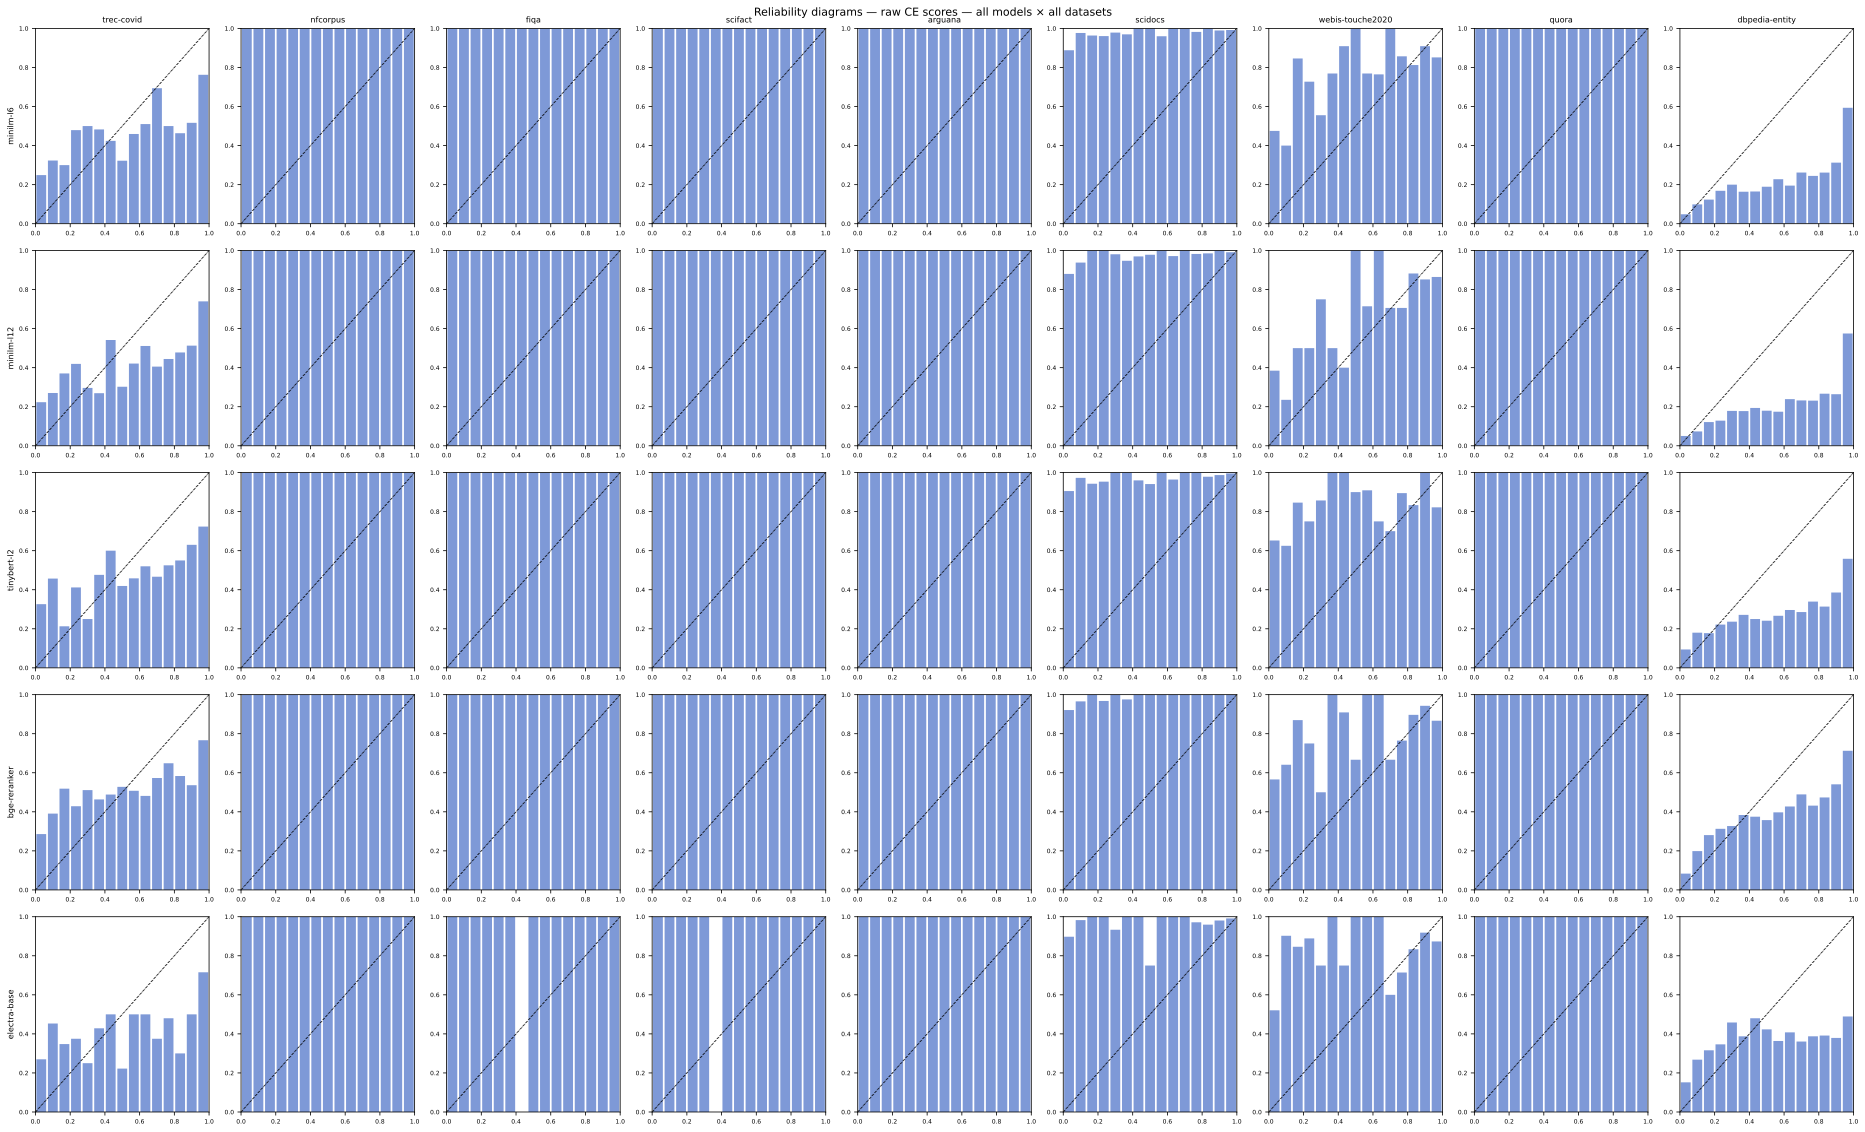
\includegraphics[width=\textwidth]{paper_all_models_all_datasets_raw.png}
\caption{Raw reliability diagrams for all five models (rows) across all nine
datasets (columns). The dashed line is perfect calibration. Bars below it mean
overconfidence. They almost all are.}
\label{fig:grid}
\end{figure}

\begin{figure}[t]
\centering
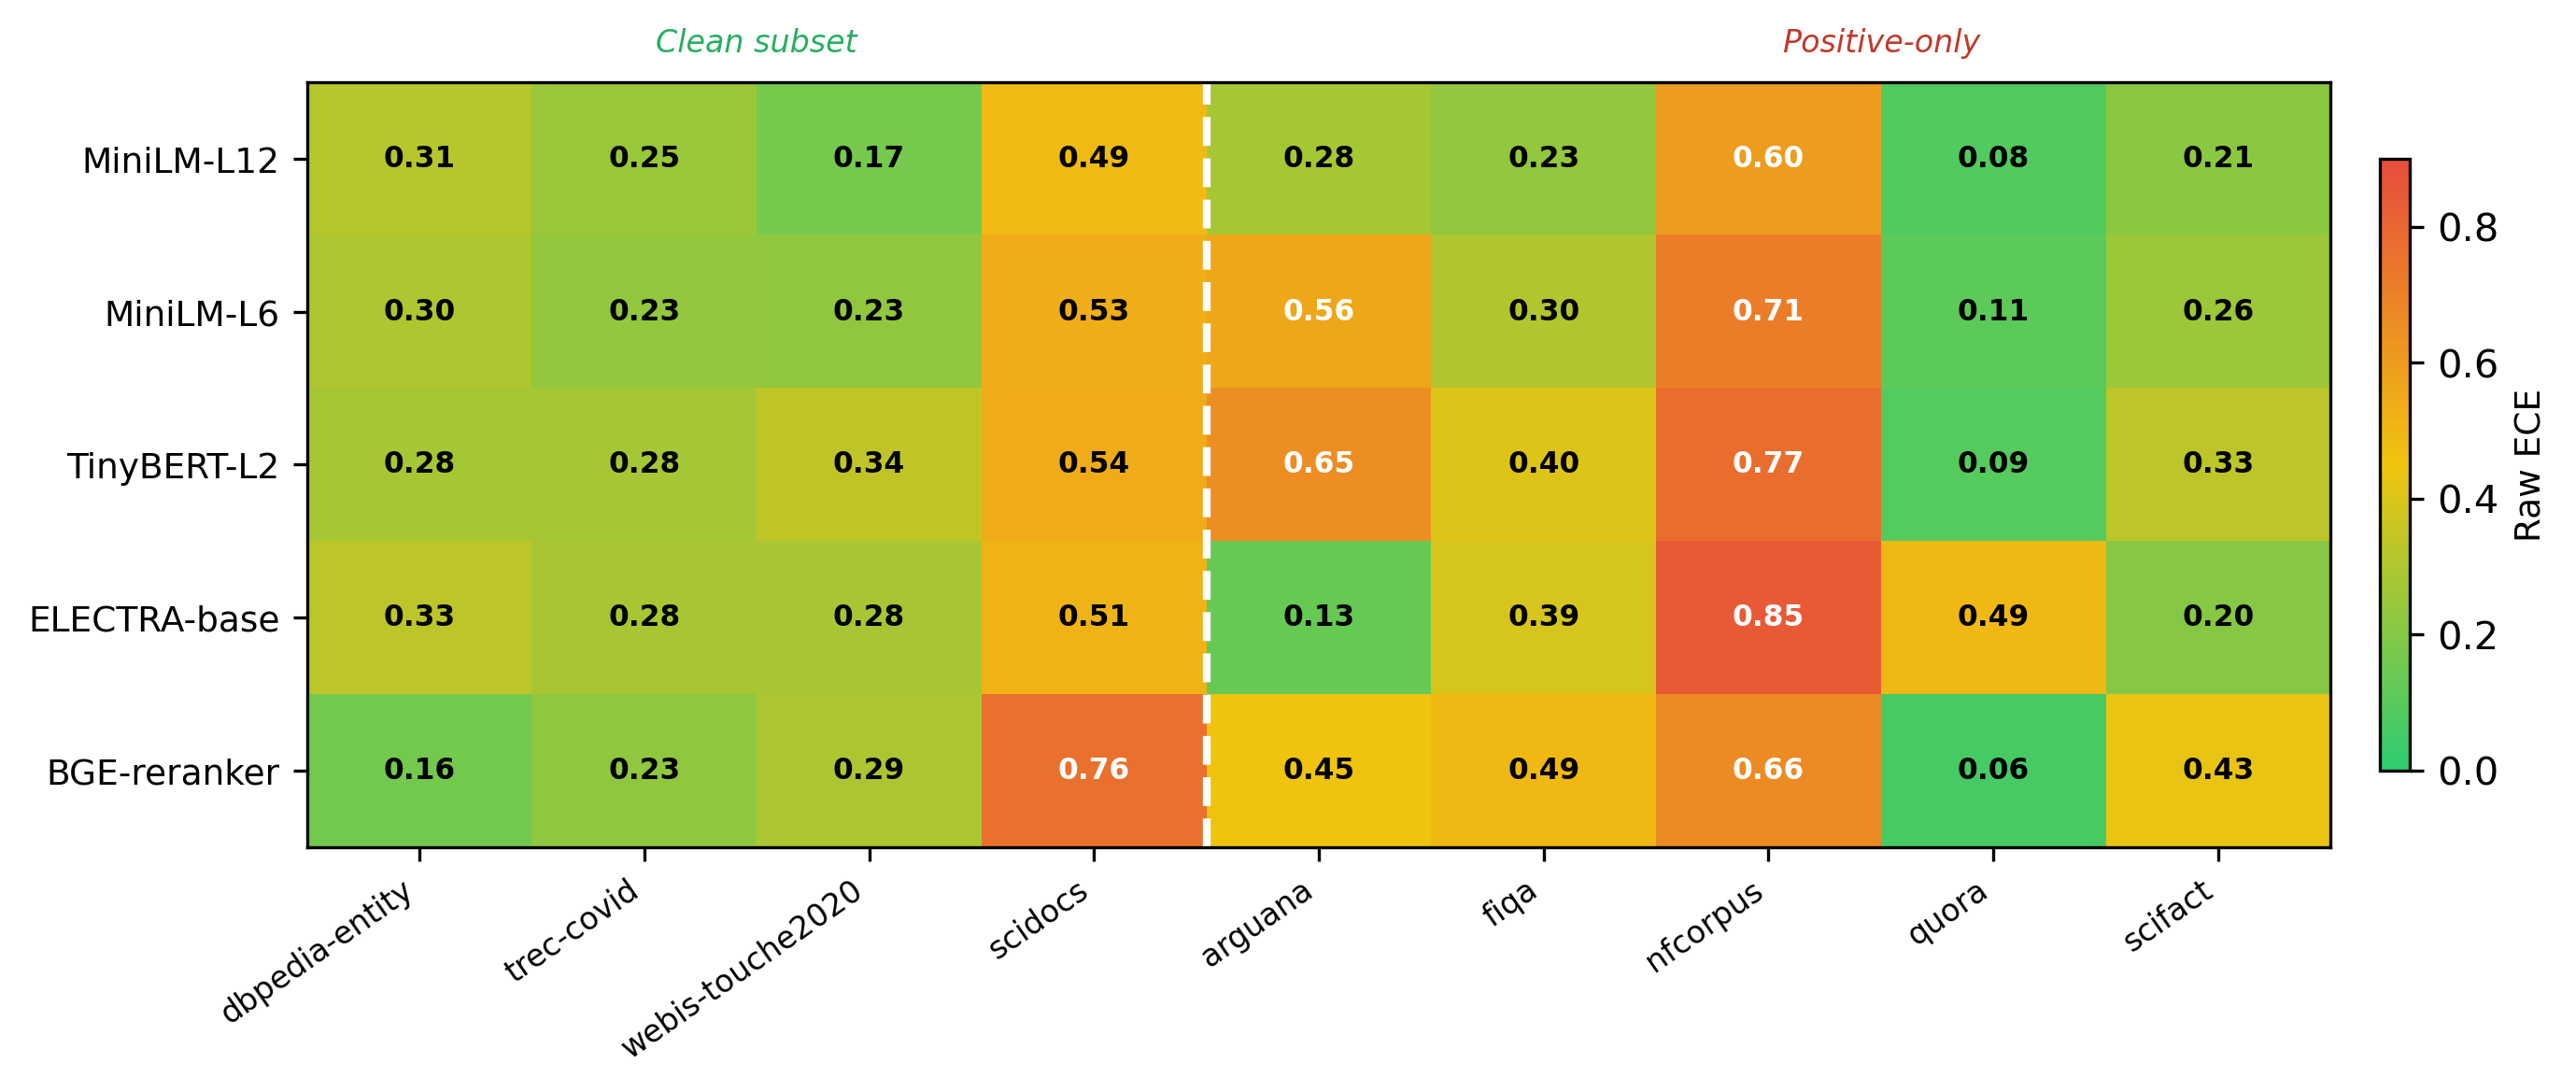
\includegraphics[width=\textwidth]{paper_fig_ece_heatmap.png}
\caption{Raw ECE as a heatmap across all model-dataset pairs. Green is low error,
red is high. The dashed line separates the clean subset (left) from the
positive-only datasets (right). The pattern is clear: overconfidence is the norm,
not the exception.}
\label{fig:heatmap}
\end{figure}

\begin{table}[t]
\centering
\caption{Raw calibration metrics per dataset (mean over five models), ordered by
prevalence. Bootstrap 95\% CIs are query-level with 1{,}000 resamples. Per-pair CIs
are released with the data.}
\label{tab:raw}
\small
\begin{tabular}{lrllrr}
\toprule
\rowcolor{headblue}
\thead{Dataset} & \thead{Prev.} & \thead{mean ECE} & \thead{95\% CI} & \thead{mean MCE} & \thead{mean Brier} \\
\midrule
\rowcolor{cleangreen}
dbpedia-entity   & 0.35 & 0.276 & [0.256, 0.297] & 0.527 & 0.290 \\
\rowcolor{cleangreen}
trec-covid       & 0.62 & 0.251 & [0.207, 0.299] & 0.409 & 0.268 \\
\rowcolor{cleangreen}
webis-touche2020 & 0.78 & 0.257 & [0.215, 0.311] & 0.675 & 0.259 \\
\rowcolor{cleangreen}
scidocs          & 0.95 & 0.562 & [0.537, 0.586] & 0.888 & 0.506 \\
\rowcolor{singleclasspink}
arguana          & 1.00 & 0.404 & [0.385, 0.422] & 0.977 & 0.314 \\
\rowcolor{singleclasspink}
fiqa             & 1.00 & 0.377 & [0.343, 0.410] & 0.983 & 0.303 \\
\rowcolor{singleclasspink}
nfcorpus         & 1.00 & 0.716 & [0.675, 0.756] & 0.991 & 0.659 \\
\rowcolor{singleclasspink}
quora            & 1.00 & 0.163 & [0.147, 0.179] & 0.976 & 0.113 \\
\rowcolor{singleclasspink}
scifact          & 1.00 & 0.308 & [0.260, 0.355] & 0.986 & 0.249 \\
\bottomrule
\end{tabular}
\end{table}

\begin{table}[t]
\centering
\caption{Per-model summary, averaged over nine datasets. $T$ is the optimal
temperature. Every model needs substantial softening ($T \gg 1$) to bring its
scores into line with reality.}
\label{tab:permodel}
\small
\begin{tabular}{lrrrr}
\toprule
\rowcolor{headblue}
\thead{Model} & \thead{Params} & \thead{mean $T$} & \thead{mean raw ECE} & \thead{mean iso ECE} \\
\midrule
\rowcolor{rowlight}
MiniLM-L12   & 33M  & 7.34  & 0.292 & 0.013 \\
\rowcolor{rowwhite}
MiniLM-L6    & 22M  & 9.57  & 0.359 & 0.012 \\
\rowcolor{rowlight}
BGE-reranker & 278M & 10.62 & 0.394 & 0.009 \\
\rowcolor{rowwhite}
ELECTRA-base & 110M & 11.60 & 0.386 & 0.012 \\
\rowcolor{rowlight}
TinyBERT-L2  & 4M   & 12.06 & 0.409 & 0.011 \\
\bottomrule
\end{tabular}
\end{table}

We should mention a practical detail. The temperature search was capped at twenty.
Fifteen of the forty-five model-dataset pairs hit that ceiling, all of them on
single-class or near-single-class data. For those pairs the reported temperature is
a lower bound; the true optimum is somewhere higher, possibly much higher, but we
cannot say where. We write these as $T \geq 20$.

One question we expected to answer cleanly was whether bigger models calibrate
better. They do not, at least not in this size range. The Spearman correlation
between parameter count and mean raw ECE is $\rho = -0.10$ ($p = 0.87$). On the
clean subset the correlation is similarly flat ($\rho = 0.30$, $p = 0.62$).
MiniLM-L12 at 33M has the lowest mean ECE, while BGE at 278M sits near the middle.
Five models are too few to draw strong conclusions, but what we can say is that size
alone does not predict calibration quality. Architecture and pretraining recipe seem
to matter more, though disentangling those effects would require a study designed
specifically for that purpose.

\subsection{The hazard: positive-only judgments break calibration evaluation}
\label{sec:hazard}

This is the part of the paper we think matters most, and it is worth walking through
carefully.

Go back to Table~\ref{tab:datasets} and look at the prevalence column again. Five
datasets sit at exactly 1.00. On those datasets, every single judged document is
relevant. There are no judged negatives. Now think about what calibration evaluation
does on such data. If a calibrator pushes all predicted probabilities toward one, it
gets an ECE near zero, because the labels are all ones and the predictions are all
near one. That is not calibration; it is pattern matching.

Isotonic regression does exactly this. On single-class fit splits it learns to map
everything to the majority class, and on the held-out split it achieves ECE of
0.000. That number looks spectacular if you do not know how it was produced. It is,
in fact, meaningless, an artifact of the evaluation setup rather than evidence of
good calibration. We want to be explicit about this because we suspect others have
been or will be tripped by it.

The harm goes beyond isotonic's inflated numbers. It contaminates the entire
comparison. If you pool all forty-five model-dataset pairs and ask how often
temperature scaling improves ECE, you get 27 out of 45, with a Wilcoxon $p = 0.024$
and a small Cohen's $d = 0.40$. That sounds disappointing. Meanwhile isotonic appears
to improve all 45. The naive conclusion is that temperature is unreliable and
isotonic is nearly magical. Both halves of that conclusion are wrong.

On single-class fit splits, the temperature optimiser has no negative examples to
learn from. The negative log-likelihood loss has no signal for pulling probabilities
down, so the temperature either drifts to the ceiling or, worse, actively moves in
the wrong direction. Figure~\ref{fig:backfire} shows this happening on scifact:
temperature scaling raises ECE instead of lowering it. On the same dataset, isotonic
regression scores 0.000 because it trivially maps everything to one. Neither result
reflects genuine calibration quality.

\begin{figure}[t]
\centering
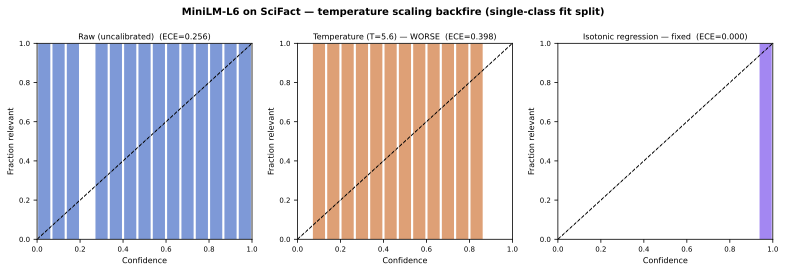
\includegraphics[width=0.85\textwidth]{paper_fig2_minilm_scifact_temp_backfire.png}
\caption{MiniLM-L6 on scifact (prevalence 1.0). Temperature scaling
\emph{worsens} ECE while isotonic regression achieves a trivial zero. Neither
number means anything; both are consequences of having no negative judgments.}
\label{fig:backfire}
\end{figure}

The right move, and really the only defensible move, is to restrict method
comparisons to datasets where the evaluation is valid. That means datasets with
genuine negative judgments. Four of ours qualify: dbpedia-entity (prevalence 0.35),
trec-covid (0.62), webis-touche2020 (0.78), and scidocs (0.95). The remaining five
are still useful for characterising the pattern of overconfidence, but they cannot
tell us which calibration fix to recommend.

\subsection{On clean data, all three methods work; a clear ranking emerges}
\label{sec:clean}

Once we restrict to the clean subset, we have twenty model-dataset pairs, and the
picture changes substantially. Table~\ref{tab:clean} reports the full results,
including all three post-hoc methods.

Start with temperature scaling. It improves ECE in all twenty pairs, with paired
$t$-test and Wilcoxon both giving $p < 0.0001$ and a large effect size of $d = 1.41$.
The mean ECE drops from about 0.34 to about 0.23. That is a real and consistent
improvement, contradicting the naive story from the pooled analysis.

Platt scaling does considerably better. It, too, improves all twenty pairs, with an
even larger effect ($d = 1.72$, $p < 0.0001$) and a mean ECE of about 0.045. That is
a fivefold improvement over temperature's 0.23, and the source of the difference is
interesting. Platt's logistic regression learns both a scale and a shift, and that
shift, the intercept term, lets it correct for systematic biases in the logit
distribution that temperature's scale-only adjustment simply cannot reach. The single
extra parameter buys a lot. Platt beats temperature head-to-head in 17 of the 20
pairs.

Isotonic regression is best of all. It improves every pair with $d = 2.02$ and brings
the mean ECE down to about 0.025. It beats Platt in 18 of 20 (Wilcoxon
$p < 0.001$). But notice the diminishing returns: the jump from temperature to Platt
(0.23 to 0.045) is much larger than the jump from Platt to isotonic (0.045 to
0.025). Whether the extra flexibility of isotonic regression is worth the overfitting
risk on small calibration sets is a judgment call that depends on deployment
conditions.

Figure~\ref{fig:fixworks} makes the progression visible on a single clean example:
BGE-reranker on trec-covid. The raw reliability bars sit well below the diagonal.
Temperature pulls them partway up. Platt and isotonic bring them close to the line.
Figure~\ref{fig:cleangrid} confirms this pattern across all models and all four clean
datasets.

\begin{figure}[t]
\centering
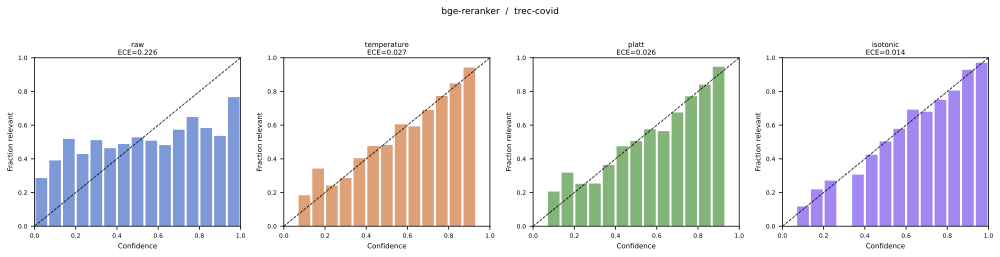
\includegraphics[width=0.95\textwidth]{paper_fig_bge_treccovid_4panel.png}
\caption{BGE-reranker on trec-covid (prevalence 0.62), four panels showing raw,
temperature, Platt, and isotonic calibration. The progression from severe
overconfidence to near-diagonal reliability bars is visible. This dataset has real
negatives, so the ECE improvements are genuine.}
\label{fig:fixworks}
\end{figure}

\begin{table}[t]
\centering
\caption{Full results on the clean subset (four datasets with genuine negatives),
held-out split. All three methods help in every pair. The ordering is consistent:
isotonic $>$ Platt $>$ temperature.}
\label{tab:clean}
\scriptsize
\setlength{\tabcolsep}{3.5pt}
\begin{tabular}{llrrrrrrr}
\toprule
\rowcolor{headblue}
\thead{Model} & \thead{Dataset} & \thead{Prev.} & \thead{raw ECE} & \thead{$T$} & \thead{temp ECE} & \thead{Platt ECE} & \thead{iso ECE} & \thead{$\Delta_{\text{iso}}$} \\
\midrule
\rowcolor{rowlight}
MiniLM-L6   & dbpedia-entity   & 0.35 & 0.297 & 5.83  & 0.219 & 0.027 & 0.024 & $-0.273$ \\
\rowcolor{rowwhite}
MiniLM-L6   & trec-covid       & 0.62 & 0.235 & 4.40  & 0.045 & 0.044 & 0.027 & $-0.208$ \\
\rowcolor{rowlight}
MiniLM-L6   & webis-touche2020 & 0.78 & 0.229 & 4.83  & 0.215 & 0.103 & 0.050 & $-0.179$ \\
\rowcolor{rowwhite}
MiniLM-L6   & scidocs          & 0.95 & 0.534 & $\geq$20 & 0.465 & 0.018 & 0.011 & $-0.523$ \\
\rowcolor{rowlight}
MiniLM-L12  & dbpedia-entity   & 0.35 & 0.313 & 6.59  & 0.221 & 0.028 & 0.019 & $-0.295$ \\
\rowcolor{rowwhite}
MiniLM-L12  & trec-covid       & 0.62 & 0.251 & 4.84  & 0.058 & 0.044 & 0.042 & $-0.209$ \\
\rowcolor{rowlight}
MiniLM-L12  & webis-touche2020 & 0.78 & 0.166 & 3.97  & 0.160 & 0.110 & 0.038 & $-0.129$ \\
\rowcolor{rowwhite}
MiniLM-L12  & scidocs          & 0.95 & 0.488 & $\geq$20 & 0.458 & 0.017 & 0.015 & $-0.472$ \\
\rowcolor{rowlight}
TinyBERT-L2 & dbpedia-entity   & 0.35 & 0.281 & 6.75  & 0.196 & 0.030 & 0.025 & $-0.256$ \\
\rowcolor{rowwhite}
TinyBERT-L2 & trec-covid       & 0.62 & 0.276 & 6.48  & 0.055 & 0.057 & 0.033 & $-0.243$ \\
\rowcolor{rowlight}
TinyBERT-L2 & webis-touche2020 & 0.78 & 0.339 & 11.08 & 0.244 & 0.060 & 0.032 & $-0.307$ \\
\rowcolor{rowwhite}
TinyBERT-L2 & scidocs          & 0.95 & 0.540 & $\geq$20 & 0.467 & 0.004 & 0.009 & $-0.532$ \\
\rowcolor{rowlight}
BGE-reranker& dbpedia-entity   & 0.35 & 0.159 & 2.96  & 0.107 & 0.028 & 0.022 & $-0.137$ \\
\rowcolor{rowwhite}
BGE-reranker& trec-covid       & 0.62 & 0.228 & 4.39  & 0.037 & 0.041 & 0.028 & $-0.199$ \\
\rowcolor{rowlight}
BGE-reranker& webis-touche2020 & 0.78 & 0.292 & 6.78  & 0.236 & 0.068 & 0.019 & $-0.274$ \\
\rowcolor{rowwhite}
BGE-reranker& scidocs          & 0.95 & 0.762 & $\geq$20 & 0.488 & 0.006 & 0.012 & $-0.751$ \\
\rowcolor{rowlight}
ELECTRA-base& dbpedia-entity   & 0.35 & 0.330 & 6.84  & 0.164 & 0.035 & 0.021 & $-0.309$ \\
\rowcolor{rowwhite}
ELECTRA-base& trec-covid       & 0.62 & 0.285 & 4.77  & 0.084 & 0.084 & 0.025 & $-0.260$ \\
\rowcolor{rowlight}
ELECTRA-base& webis-touche2020 & 0.78 & 0.283 & 6.10  & 0.249 & 0.068 & 0.052 & $-0.231$ \\
\rowcolor{rowwhite}
ELECTRA-base& scidocs          & 0.95 & 0.512 & $\geq$20 & 0.466 & 0.019 & 0.008 & $-0.504$ \\
\midrule
\rowcolor{cleangreen}
\multicolumn{3}{l}{\textbf{Mean (clean)}} & \textbf{0.340} & & \textbf{0.232} & \textbf{0.045} & \textbf{0.025} & \\
\bottomrule
\end{tabular}
\end{table}

\begin{figure}[t]
\centering
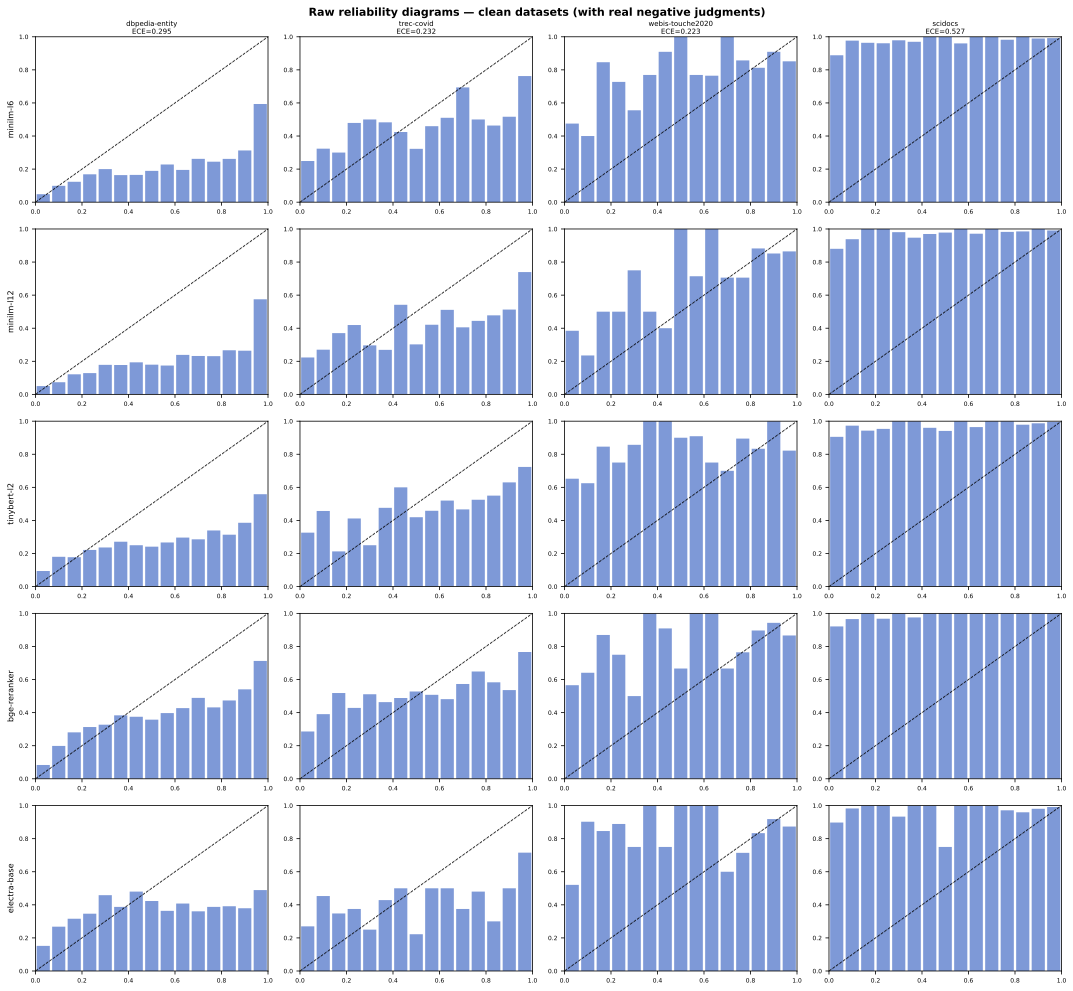
\includegraphics[width=\textwidth]{paper_fig3_all_models_clean_datasets.png}
\caption{Raw reliability diagrams on the clean subset: five models by four datasets
with real negatives. The consistent gap below the diagonal is overconfidence on data
where that label actually means something.}
\label{fig:cleangrid}
\end{figure}

Two qualifications need stating here, and they come up again in
Section~\ref{sec:limits}. The clean subset is small. Four datasets is not many, and
within those four, scidocs is near-single-class at prevalence 0.95 (its temperatures
hit the ceiling), and webis-touche2020 has only forty-nine queries, which means its
bootstrap intervals are wide enough to be uncomfortable. The two datasets we feel
most confident about are dbpedia-entity and trec-covid.

\subsection{Calibration does not cost anything in ranking quality}
\label{sec:downstream}

One concern a practitioner might raise is that fixing calibration could break
ranking. It does not. Because all three methods are monotone transforms, they
cannot reorder documents. Table~\ref{tab:downstream} confirms this empirically:
the maximum absolute change in nDCG@10 across all forty-five pairs is
$1.0 \times 10^{-4}$, which is essentially zero. Calibration is, in a real sense,
free.

\begin{table}[t]
\centering
\caption{Downstream ranking metrics per dataset (mean over five models). nDCG@10
and MAP are unchanged after calibration. The accept rate at $p > 0.5$ is also
unchanged, because even after dividing logits by $T \approx 10$, most scores remain
above 0.5.}
\label{tab:downstream}
\small
\begin{tabular}{lrrrr}
\toprule
\rowcolor{headblue}
\thead{Dataset} & \thead{nDCG@10} & \thead{MAP} & \thead{Accept (raw)} & \thead{Accept (cal)} \\
\midrule
\rowcolor{cleangreen}
dbpedia-entity   & 0.349 & 0.455 & 0.963 & 0.963 \\
\rowcolor{cleangreen}
trec-covid       & 0.686 & 0.680 & 0.988 & 0.988 \\
\rowcolor{cleangreen}
webis-touche2020 & 0.265 & 0.287 & 0.988 & 0.988 \\
\rowcolor{cleangreen}
scidocs          & 0.157 & 0.214 & 0.797 & 0.797 \\
\rowcolor{singleclasspink}
arguana          & 0.253 & 0.181 & 1.000 & 1.000 \\
\rowcolor{singleclasspink}
fiqa             & 0.316 & 0.352 & 0.827 & 0.827 \\
\rowcolor{singleclasspink}
nfcorpus         & 0.315 & 0.389 & 0.599 & 0.599 \\
\rowcolor{singleclasspink}
quora            & 0.780 & 0.751 & 0.922 & 0.922 \\
\rowcolor{singleclasspink}
scifact          & 0.676 & 0.644 & 0.805 & 0.805 \\
\bottomrule
\end{tabular}
\end{table}

There is, however, a subtlety worth flagging for anyone building threshold-based
systems. At a typical abstention threshold of $p > 0.5$, the accept rate does not
change after temperature scaling in any of the forty-five pairs. The reason is
almost ironic: the models are \emph{so} overconfident that even dividing the logit
by ten leaves most scores above 0.5. Calibration makes the numbers honest, but it
does not, on its own, rescue a hard probability gate from models this far off. You
would need either a non-monotone correction or a re-tuned threshold, both of which
are outside the scope of what we tried here.

% =============================================================================
\section{Sensitivity Analysis}
\label{sec:sensitivity}

A reviewer might reasonably ask: why restrict to judged pairs? In deployment,
unjudged documents get shown to users. They are not filtered out. To address this,
we recomputed ECE under an alternative convention where every unjudged pair is
treated as non-relevant.

The result is instructive but not cleanly interpretable. The mean ECE shifts by
$-0.167$ across the forty-five pairs, but the direction is inconsistent: ECE drops in
28 pairs and rises in 17. Which way it goes is driven entirely by dataset structure.
On positive-only datasets, adding a flood of ``negative'' unjudged pairs dilutes the
relevant mass, making the model look better calibrated. On datasets that already have
real negatives, the extra pseudo-negatives make things look worse. The pattern
reinforces exactly the point from Section~\ref{sec:hazard}: there is no
assumption-free calibration number on BEIR. The judgment structure shapes the
metric, and it has to be reported alongside any ECE.

We use judged-only as the primary convention, which is standard, and note that the
conclusions from the clean subset hold under both treatments.

% =============================================================================
\section{Discussion}
\label{sec:discussion}

\paragraph{A deployment recipe.}
If you are running one of these re-rankers and consuming its sigmoid output as a
probability, the practical advice is simple: do not trust those numbers without
correction. Table~\ref{tab:recipe} gives a concrete recipe. For each model, we
report the mean optimal temperature computed on the clean subset. Dividing the logit
by that temperature before the sigmoid is a one-line code change, requires no
retraining, and brings the probabilities substantially closer to reality.

\begin{table}[t]
\centering
\caption{Deployment recipe: recommended temperature per model, computed as the mean
optimal $T$ on the clean subset. Apply by dividing the logit by $T$ before the
sigmoid. The range reflects domain variability.}
\label{tab:recipe}
\small
\begin{tabular}{lrrrr}
\toprule
\rowcolor{headblue}
\thead{Model} & \thead{Params} & \thead{Rec.\ $T$} & \thead{$T$ range} & \thead{Clean ECE (raw $\to$ temp)} \\
\midrule
\rowcolor{rowlight}
BGE-reranker & 278M & 8.53  & [2.96, $\geq$20] & 0.360 $\to$ 0.217 \\
\rowcolor{rowwhite}
MiniLM-L6    & 22M  & 8.77  & [4.40, $\geq$20] & 0.324 $\to$ 0.236 \\
\rowcolor{rowlight}
MiniLM-L12   & 33M  & 8.85  & [3.97, $\geq$20] & 0.305 $\to$ 0.224 \\
\rowcolor{rowwhite}
ELECTRA-base & 110M & 9.43  & [4.77, $\geq$20] & 0.352 $\to$ 0.241 \\
\rowcolor{rowlight}
TinyBERT-L2  & 4M   & 11.08 & [6.48, $\geq$20] & 0.359 $\to$ 0.241 \\
\bottomrule
\end{tabular}
\end{table}

Where you have a held-out calibration set with real negatives, Platt scaling or
isotonic regression will do better, often much better. The temperatures above are
a floor, not a ceiling.

\paragraph{Platt scaling deserves more attention than it gets.}
One result that surprised us was how well Platt scaling performs on the clean data.
With a mean ECE of 0.045, it lands roughly five times closer to perfect calibration
than temperature scaling's 0.23. The difference comes down to a single parameter:
the intercept. Temperature can scale the logits, but it cannot shift the operating
point. Platt can. That shift turns out to matter quite a bit for cross-encoder logit
distributions, which may not be centered where the sigmoid expects them to be.
Isotonic regression does better still, reaching 0.025, but the gap between Platt
and isotonic is much tighter than the gap between temperature and Platt. In
deployment scenarios where the calibration set is small and you worry about
overfitting, Platt might well be the pragmatic sweet spot.

\paragraph{BGE-reranker stands out.}
On dbpedia-entity, the most balanced of our clean datasets, BGE-reranker is the
best-calibrated model out of the box (raw ECE 0.159) and needs the gentlest
correction ($T = 2.96$, compared to the others at six or above). Whether this is a
consequence of its larger capacity, its XLM-RoBERTa backbone, or its contrastive
pretraining, we genuinely cannot tell. The absence of any size-calibration
correlation ($\rho = -0.10$) suggests it is not simply a matter of having more
parameters, but pinning down the mechanism would require controlled experiments that
are beyond what we attempted.

\paragraph{For anyone evaluating calibration on BEIR.}
The methodological lesson is concrete and, we believe, broadly applicable: report
qrel prevalence whenever you measure calibration on BEIR datasets. Restrict
method comparisons to datasets with genuine negatives. Without this, a study can
produce statistically significant but entirely wrong conclusions about which
calibration method to trust. Our own naive analysis demonstrates exactly how
convincingly wrong those conclusions can look.

% =============================================================================
\section{Limitations}
\label{sec:limits}

We would rather state these ourselves than have a reviewer discover them.

The most obvious limitation is that five of nine datasets have positive-only
judgments. Their ECE is not a meaningful measure of calibration in any interpretable
sense. We exclude them from method comparisons and use them only to document the
pattern of overconfidence and to illustrate the evaluation hazard. Isotonic
regression's ECE of zero on these datasets is an artifact, and we have said so
repeatedly rather than hoping nobody notices.

The clean subset is small and not perfectly balanced. Four datasets is not a lot, and
within those four, scidocs sits at prevalence 0.95 (nearly single-class) and hits
the temperature ceiling, while webis-touche2020 has only forty-nine queries. Wide
bootstrap confidence intervals on forty-nine queries are not reassuring. The two
anchors we trust most are dbpedia-entity and trec-covid. A study with more
well-balanced IR datasets would be welcome.

Several reported temperatures are lower bounds rather than point estimates. The
optimiser was capped at twenty, and fifteen of forty-five pairs hit that cap. We
do not know how much higher the true optima go.

The model scope covers 4M to 278M parameters. We did not study larger re-rankers
like BGE-large or LLM-based re-rankers such as RankLLaMA~\cite{ma2024rankllama}, and
there is no guarantee our findings transfer. Calibration behaviour could be quite
different at the billion-parameter scale.

All five models were trained on MS~MARCO. What happens with re-rankers trained on
other data, or on mixtures, is unknown. The jina-reranker-v1-tiny-en exclusion due
to software incompatibility is a minor gap but worth noting for completeness.

ECE itself has known issues. Our choice of fifteen equal-width bins is one of many
possible schemes, and different binning can give different
results~\cite{nixon2019}. We treated the binning as fixed rather than tuning it,
which avoids one kind of bias at the cost of possibly introducing another. Adaptive
binning and kernel-based calibration metrics are natural extensions.

Finally, Quora was subsampled to 1{,}000 queries for computational cost, which means
our numbers for that dataset are noisier than they would be on the full 10{,}000.

% =============================================================================
\section{Conclusion}
\label{sec:conclusion}

Cross-encoder re-rankers are overconfident. Every model we tested, on every domain
where the measurement is meaningful, produces scores that are systematically too
high. Optimal temperatures run from roughly three to above twenty, which means the
raw sigmoid output of these models is not a probability in any useful sense.

The standard way to evaluate calibration on BEIR is broken by positive-only
judgments, and that breakage creates misleading narratives. Temperature scaling
looks unreliable when it is not. Isotonic regression looks magical when it is just
exploiting a degenerate evaluation. The fix is straightforward but not widely
practiced: report prevalence, restrict method comparisons to datasets with real
negatives.

When the evaluation is valid, calibration works and it is free. All three
post-hoc methods improve calibration without disturbing the ranking. A clear
ordering emerges: isotonic is best, Platt is close behind (and may be the
better practical choice on small calibration sets), and temperature is the
simplest option that still helps substantially. We release the scored data, the
fitted calibrators, and the code, and we point to abstention-aware calibration,
larger re-rankers, and per-query calibration as directions worth exploring next.

% =============================================================================
\section*{Reproducibility}
All code, scored pairs, per-model fitted temperatures, Platt parameters, and
reliability diagrams are available at \url{https://github.com/Codewithsayanjib/CalRank}. The pipeline is
deterministic (seed 42), runs on an Apple~M4, and is designed to be resumable.
Released artifacts include: raw calibration metrics with bootstrap confidence
intervals, post-hoc calibration results for all three methods, fitted calibration
parameters as a drop-in deployment recipe, the clean-subset analysis, the
sensitivity analysis under unjudged-as-negative treatment, and all reliability
diagrams in both PDF and PNG formats.

% =============================================================================
\bibliographystyle{plain}
\begin{thebibliography}{30}

\bibitem{bm25s2024} X.~Lu.
BM25S: Orders of magnitude faster lexical search via eager sparse scoring.
\emph{arXiv:2407.03618}, 2024.

\bibitem{brier1950} G.~W. Brier.
Verification of forecasts expressed in terms of probability.
\emph{Monthly Weather Review}, 78(1):1--3, 1950.

\bibitem{clark2020electra} K.~Clark, M.-T. Luong, Q.~V. Le, C.~D. Manning.
ELECTRA: Pre-training text encoders as discriminators rather than generators.
\emph{ICLR}, 2020.

\bibitem{craswell2020} N.~Craswell, B.~Mitra, E.~Yilmaz, D.~Campos.
Overview of the TREC 2020 Deep Learning Track.
\emph{Proceedings of TREC}, 2020.

\bibitem{degroot1983} M.~H. DeGroot, S.~E. Fienberg.
The comparison and evaluation of forecasters.
\emph{The Statistician}, 32(1-2):12--22, 1983.

\bibitem{desai2020} S.~Desai, G.~Durrett.
Calibration of pre-trained transformers.
\emph{EMNLP}, 2020.

\bibitem{el2010} Y.~El-Yaniv, Y.~Wiener.
On the foundations of noise-free selective classification.
\emph{JMLR}, 11:1605--1646, 2010.

\bibitem{gao2024rag} Y.~Gao, Y.~Xiong, A.~Dixit, et al.
Retrieval-augmented generation for large language models: A survey.
\emph{arXiv:2312.10997}, 2024.

\bibitem{geifman2017} Y.~Geifman, R.~El-Yaniv.
Selective classification for deep neural networks.
\emph{NeurIPS}, 2017.

\bibitem{guo2017} C.~Guo, G.~Pleiss, Y.~Sun, K.~Q. Weinberger.
On calibration of modern neural networks.
\emph{ICML}, 2017.

\bibitem{jiang2021} Z.~Jiang, J.~Araki, H.~Ding, G.~Neubig.
How can we know when language models know? On the calibration of language models
for question answering.
\emph{TACL}, 9:962--977, 2021.

\bibitem{jiao2020tinybert} X.~Jiao, Y.~Yin, L.~Shang, X.~Jiang, X.~Chen,
L.~Li, F.~Wang, Q.~Liu.
TinyBERT: Distilling BERT for natural language understanding.
\emph{Findings of EMNLP}, 2020.

\bibitem{kadavath2022} S.~Kadavath, T.~Conerly, A.~Askell, et al.
Language models (mostly) know what they know.
\emph{arXiv:2207.05221}, 2022.

\bibitem{kumar2019} A.~Kumar, S.~Sarawagi, U.~Jain.
Trainable calibration measures for neural networks from kernel mean embeddings.
\emph{ICML}, 2019.

\bibitem{lewis2020rag} P.~Lewis, E.~Perez, A.~Piktus, et al.
Retrieval-augmented generation for knowledge-intensive NLP tasks.
\emph{NeurIPS}, 2020.

\bibitem{lin2021pyserini} J.~Lin, X.~Ma, S.-C. Lin, J.-H. Yang, R.~Pradeep,
R.~Nogueira.
Pyserini: A Python toolkit for reproducible information retrieval research with
sparse and dense representations.
\emph{SIGIR}, 2021.

\bibitem{ma2024rankllama} X.~Ma, L.~Gao, J.~Callan.
Fine-tuning LLaMA for multi-stage text retrieval.
\emph{SIGIR}, 2024.

\bibitem{naeini2015} M.~P. Naeini, G.~F. Cooper, M.~Hauskrecht.
Obtaining well calibrated probabilities using Bayesian binning into quantiles.
\emph{AAAI}, 2015.

\bibitem{nguyen2016msmarco} T.~Nguyen, M.~Rosenberg, X.~Song, J.~Gao,
S.~Tiwary, R.~Majumder, L.~Deng.
MS MARCO: A human generated machine reading comprehension dataset.
\emph{NeurIPS Workshop on Cognitive Computation}, 2016.

\bibitem{niculescu2005} A.~Niculescu-Mizil, R.~Caruana.
Predicting good probabilities with supervised learning.
\emph{ICML}, 2005.

\bibitem{nixon2019} J.~Nixon, M.~W. Dusenberry, L.~Zhang, G.~Jerfel,
D.~Tran.
Measuring calibration in deep learning.
\emph{CVPR Workshops}, 2019.

\bibitem{nogueira2019} R.~Nogueira, K.~Cho.
Passage re-ranking with BERT.
\emph{arXiv:1901.04085}, 2019.

\bibitem{platt1999} J.~Platt.
Probabilistic outputs for support vector machines and comparisons to regularized
likelihood methods.
\emph{Advances in Large Margin Classifiers}, 1999.

\bibitem{reimers2019sbert} N.~Reimers, I.~Gurevych.
Sentence-BERT: Sentence embeddings using Siamese BERT-networks.
\emph{EMNLP}, 2019.

\bibitem{robertson2009bm25} S.~Robertson, H.~Zaragoza.
The probabilistic relevance framework: BM25 and beyond.
\emph{Foundations and Trends in Information Retrieval}, 3(4):333--389, 2009.

\bibitem{thakur2021beir} N.~Thakur, N.~Reimers, A.~R\"uckl\'e, A.~Srivastava,
I.~Gurevych.
BEIR: A heterogeneous benchmark for zero-shot evaluation of information retrieval
models.
\emph{NeurIPS Datasets and Benchmarks}, 2021.

\bibitem{tian2023} K.~Tian, E.~Mitchell, A.~Yao, C.~D. Manning, C.~Finn.
Just ask for calibration: Strategies for eliciting calibrated confidence scores
from language models fine-tuned with human feedback.
\emph{EMNLP}, 2023.

\bibitem{wang2020minilm} W.~Wang, F.~Wei, L.~Dong, H.~Bao, N.~Yang, M.~Zhou.
MiniLM: Deep self-attention distillation for task-agnostic compression of
pre-trained transformers.
\emph{NeurIPS}, 2020.

\bibitem{xiao2023bge} S.~Xiao, Z.~Liu, P.~Zhang, N.~Muennighoff.
C-Pack: Packed resources for general Chinese embeddings.
\emph{arXiv:2309.07597}, 2023.

\bibitem{zadrozny2002} B.~Zadrozny, C.~Elkan.
Transforming classifier scores into accurate multiclass probability estimates.
\emph{KDD}, 2002.

\end{thebibliography}

% =============================================================================
\clearpage
\appendix
\section{Full Results: All 45 Model-Dataset Pairs}
\label{app:full}

Table~\ref{tab:full} reports everything. Platt scaling is marked ``---'' where the
fit fails due to single-class data. Isotonic ECE of 0.000 on prevalence-one datasets
is an artifact, not a result, as discussed at length in Section~\ref{sec:hazard}.

\begin{table}[h!]
\centering
\caption{Complete calibration results for all 45 model-dataset pairs (held-out
split). Platt ``---'' indicates inapplicability on single-class data. Isotonic
ECE of 0.000 at prevalence 1.00 is an artifact.}
\label{tab:full}
\scriptsize
\setlength{\tabcolsep}{3pt}
\begin{tabular}{llrrrrrrr}
\toprule
\rowcolor{headblue}
\thead{Model} & \thead{Dataset} & \thead{Prev.} & \thead{raw ECE} & \thead{$T$} & \thead{temp ECE} & \thead{Platt ECE} & \thead{iso ECE} \\
\midrule
\rowcolor{cleangreen}
MiniLM-L6      & dbpedia-entity       & 0.35 & 0.297 & 5.83 & 0.219 & 0.027 & 0.024 \\
\rowcolor{cleangreen}
MiniLM-L6      & trec-covid           & 0.62 & 0.235 & 4.40 & 0.045 & 0.044 & 0.027 \\
\rowcolor{cleangreen}
MiniLM-L6      & webis-touche2020     & 0.78 & 0.229 & 4.83 & 0.215 & 0.103 & 0.050 \\
\rowcolor{cleangreen}
MiniLM-L6      & scidocs              & 0.95 & 0.534 & $\geq$20 & 0.464 & 0.018 & 0.011 \\
\rowcolor{singleclasspink}
MiniLM-L6      & arguana              & 1.00 & 0.558 & $\geq$20 & 0.507 & --- & 0.000 \\
\rowcolor{singleclasspink}
MiniLM-L6      & fiqa                 & 1.00 & 0.302 & 4.36 & 0.400 & --- & 0.000 \\
\rowcolor{singleclasspink}
MiniLM-L6      & nfcorpus             & 1.00 & 0.712 & $\geq$20 & 0.537 & --- & 0.000 \\
\rowcolor{singleclasspink}
MiniLM-L6      & quora                & 1.00 & 0.107 & 1.13 & 0.114 & --- & 0.000 \\
\rowcolor{singleclasspink}
MiniLM-L6      & scifact              & 1.00 & 0.256 & 5.57 & 0.398 & --- & 0.000 \\
\midrule
\rowcolor{cleangreen}
MiniLM-L12     & dbpedia-entity       & 0.35 & 0.313 & 6.59 & 0.221 & 0.028 & 0.019 \\
\rowcolor{cleangreen}
MiniLM-L12     & trec-covid           & 0.62 & 0.251 & 4.84 & 0.058 & 0.044 & 0.042 \\
\rowcolor{cleangreen}
MiniLM-L12     & webis-touche2020     & 0.78 & 0.166 & 3.97 & 0.160 & 0.110 & 0.038 \\
\rowcolor{cleangreen}
MiniLM-L12     & scidocs              & 0.95 & 0.488 & $\geq$20 & 0.458 & 0.017 & 0.015 \\
\rowcolor{singleclasspink}
MiniLM-L12     & arguana              & 1.00 & 0.278 & 2.43 & 0.349 & --- & 0.000 \\
\rowcolor{singleclasspink}
MiniLM-L12     & fiqa                 & 1.00 & 0.233 & 2.81 & 0.316 & --- & 0.000 \\
\rowcolor{singleclasspink}
MiniLM-L12     & nfcorpus             & 1.00 & 0.601 & $\geq$20 & 0.521 & --- & 0.000 \\
\rowcolor{singleclasspink}
MiniLM-L12     & quora                & 1.00 & 0.082 & 1.11 & 0.087 & --- & 0.000 \\
\rowcolor{singleclasspink}
MiniLM-L12     & scifact              & 1.00 & 0.215 & 4.30 & 0.344 & --- & 0.000 \\
\midrule
\rowcolor{cleangreen}
TinyBERT-L2    & dbpedia-entity       & 0.35 & 0.281 & 6.75 & 0.196 & 0.030 & 0.025 \\
\rowcolor{cleangreen}
TinyBERT-L2    & trec-covid           & 0.62 & 0.276 & 6.48 & 0.055 & 0.057 & 0.033 \\
\rowcolor{cleangreen}
TinyBERT-L2    & webis-touche2020     & 0.78 & 0.339 & 11.08 & 0.244 & 0.060 & 0.032 \\
\rowcolor{cleangreen}
TinyBERT-L2    & scidocs              & 0.95 & 0.540 & $\geq$20 & 0.467 & 0.004 & 0.009 \\
\rowcolor{singleclasspink}
TinyBERT-L2    & arguana              & 1.00 & 0.648 & $\geq$20 & 0.524 & --- & 0.000 \\
\rowcolor{singleclasspink}
TinyBERT-L2    & fiqa                 & 1.00 & 0.405 & 15.87 & 0.485 & --- & 0.000 \\
\rowcolor{singleclasspink}
TinyBERT-L2    & nfcorpus             & 1.00 & 0.767 & $\geq$20 & 0.552 & --- & 0.000 \\
\rowcolor{singleclasspink}
TinyBERT-L2    & quora                & 1.00 & 0.092 & 2.11 & 0.119 & --- & 0.000 \\
\rowcolor{singleclasspink}
TinyBERT-L2    & scifact              & 1.00 & 0.329 & 6.27 & 0.424 & --- & 0.000 \\
\midrule
\rowcolor{cleangreen}
BGE-reranker   & dbpedia-entity       & 0.35 & 0.159 & 2.96 & 0.107 & 0.028 & 0.022 \\
\rowcolor{cleangreen}
BGE-reranker   & trec-covid           & 0.62 & 0.228 & 4.39 & 0.037 & 0.041 & 0.028 \\
\rowcolor{cleangreen}
BGE-reranker   & webis-touche2020     & 0.78 & 0.292 & 6.78 & 0.236 & 0.068 & 0.019 \\
\rowcolor{cleangreen}
BGE-reranker   & scidocs              & 0.95 & 0.762 & $\geq$20 & 0.488 & 0.006 & 0.012 \\
\rowcolor{singleclasspink}
BGE-reranker   & arguana              & 1.00 & 0.453 & 8.70 & 0.490 & --- & 0.000 \\
\rowcolor{singleclasspink}
BGE-reranker   & fiqa                 & 1.00 & 0.494 & $\geq$20 & 0.499 & --- & 0.000 \\
\rowcolor{singleclasspink}
BGE-reranker   & nfcorpus             & 1.00 & 0.665 & $\geq$20 & 0.525 & --- & 0.000 \\
\rowcolor{singleclasspink}
BGE-reranker   & quora                & 1.00 & 0.058 & 1.10 & 0.061 & --- & 0.000 \\
\rowcolor{singleclasspink}
BGE-reranker   & scifact              & 1.00 & 0.435 & 11.68 & 0.483 & --- & 0.000 \\
\midrule
\rowcolor{cleangreen}
ELECTRA-base   & dbpedia-entity       & 0.35 & 0.330 & 6.84 & 0.164 & 0.035 & 0.021 \\
\rowcolor{cleangreen}
ELECTRA-base   & trec-covid           & 0.62 & 0.285 & 4.77 & 0.084 & 0.084 & 0.025 \\
\rowcolor{cleangreen}
ELECTRA-base   & webis-touche2020     & 0.78 & 0.283 & 6.10 & 0.249 & 0.068 & 0.052 \\
\rowcolor{cleangreen}
ELECTRA-base   & scidocs              & 0.95 & 0.512 & $\geq$20 & 0.466 & 0.019 & 0.008 \\
\rowcolor{singleclasspink}
ELECTRA-base   & arguana              & 1.00 & 0.131 & 1.31 & 0.161 & --- & 0.000 \\
\rowcolor{singleclasspink}
ELECTRA-base   & fiqa                 & 1.00 & 0.387 & $\geq$20 & 0.493 & --- & 0.000 \\
\rowcolor{singleclasspink}
ELECTRA-base   & nfcorpus             & 1.00 & 0.846 & $\geq$20 & 0.561 & --- & 0.000 \\
\rowcolor{singleclasspink}
ELECTRA-base   & quora                & 1.00 & 0.495 & $\geq$20 & 0.502 & --- & 0.000 \\
\rowcolor{singleclasspink}
ELECTRA-base   & scifact              & 1.00 & 0.205 & 5.38 & 0.404 & --- & 0.000 \\
\bottomrule
\end{tabular}
\end{table}

\end{document}
